\documentclass{standalone}
\usepackage{tikz}
\usetikzlibrary{decorations.pathmorphing,patterns}
\begin{document}
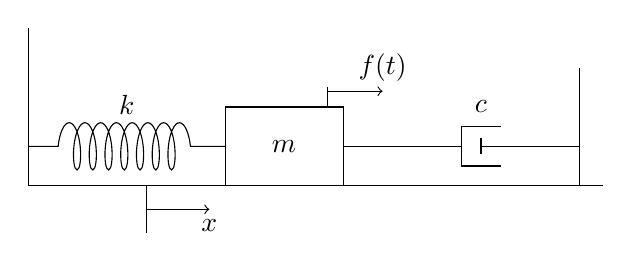
\begin{tikzpicture}
\draw (-2,0) -- (5.3,0);
\draw (-2,0) -- (-2,2);
\draw (-0.5,0) -- (-0.5,-0.6);
\draw [->] (-0.5,-0.3) -- (0.3,-0.3);
\draw (0.3,-0.5) node {$x$};
\draw[decoration={aspect=0.3, pre length = 3.8mm, post length =3mm, segment length=2mm, amplitude=3mm,coil},decorate] (-2,0.5) -- (0.5,0.5) node [midway, above = 8] {$k$}; 
\draw (0.5,0) rectangle (2, 1) node [pos=0.5] {$m$};
\draw (2,0.5) -- (3.5,0.5);
\draw (3.5, 0.25) -- (3.5,0.75);
\draw (3.5,0.75) -- (4,0.75);
\draw (3.5,0.25) -- (4,0.25);
\draw (3.75,0.6) -- (3.75,0.4);
\draw (3.75,0.5) -- (5,0.5);
\draw (5,0) -- (5,1.5);
\draw (2.5, 1.5) node {$f(t)$};
\draw [->] (1.8,1.2) -- (2.5,1.2);
\draw (1.8,1) -- (1.8,1.25);
\draw (3.75, 1) node {$c$};
\end{tikzpicture}
\end{document}